
\subsection{Bi-objective optimization}

Assume that you want to minimize two objectives (ex: risk and cost).
Objective are not always comparable often conflicting.

\begin{itemize}
    \item \textbf{Lexicographic optimization}: You consider that one of
        the objective is much more important than the other one.

        For example, in vehicle routing, we prefer (6trucks, 500km) rather
        than (7trucks, 250km) because driver are costly than kilometers.

        \begin{enumerate}
            \item Minimize the first objective and found $T*$ the number
                of trucks

                \textit{In practive done with column generation for
                instance}
            \item Minize the second objective according to 
                the first minimization, so number of trucks $\leq T*$

                \textit{In practice, use local search to improve
                solution generated by column generation}
        \end{enumerate}

    \item \textbf{Weighted objective}: Monetize each objective. 
        The problem is that you don’t always have these costs,
        and you may want to generate \textit{candidate} solutions
        event before these costs are known.

    \item \textbf{Dominance}
        \begin{center}
            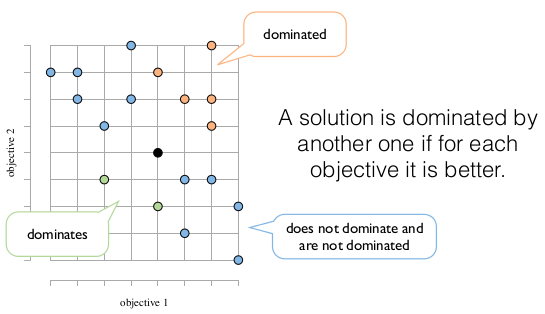
\includegraphics[width=11cm]{dominance}
        \end{center}

\end{itemize}


\subsubsection{Pareto set (efficient set)}
A solution is efficient iff it is not dominated by any
satisfiable solution. The goal if to discover the \textbf{Pareto set}
without considering every possibles feasible solutions.

\begin{itemize}
    \item \textbf{Weighted Sum}:  Find point on the \textbf{convex hull}
        of the pareto front for the bi-objective 

        \begin{lstlisting}[mathescape]
step = 0.1
$\alpha = 0$
setPareto = $\emptyset$
while $\alpha < 1$ do
    minimize $\alpha * obj_1 + (1-\alpha) * obj_2$
    setPareto = setPareto $\cup (obj_1*, obj_2*)$
    $\alpha +=$ step
    \end{lstlisting}

    \begin{tabular}{m{10cm}m{6cm}}
        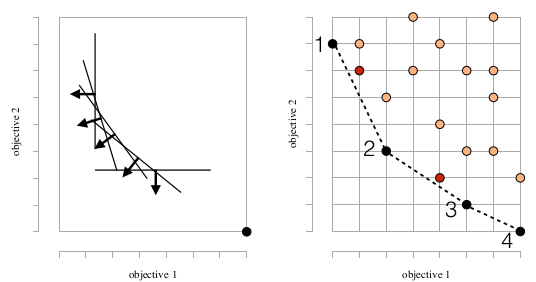
\includegraphics[width=10cm]{weighted}
        &
        \begin{itemize}
            \item As only the convex hull of the pareto front can be
                discover, some points (red) can be miss in the concave parts
        \end{itemize}
    \end{tabular}

    $\Rightarrow$ \begin{tabular}{l}
        Only discover subset of points on the convex hull\\
        Can be generalized to more than two objective\\
        $\alpha$ not easy to find (too small $\alpha$ will rediscover
        the same solution several times)
        \end{tabular}

    \item \textbf{Epsilon constraint}: Find pareto front for the
        bi-objective

        \begin{lstlisting}[mathescape]
$\epsilon$ = 0.1
setPareto = $\emptyset$
$o_2 = \infty$
ok = true
while ok do
    ok = false
    minimize $obj_1$ subject to $obj_2 \leq o_2* - \epsilon$
    if solution found then
        ok = true
        setPareto = setPareto $\cup (obj_1*, obj_2*)$
        $o_2 = obj_2*$
    \end{lstlisting}

    \begin{center}
        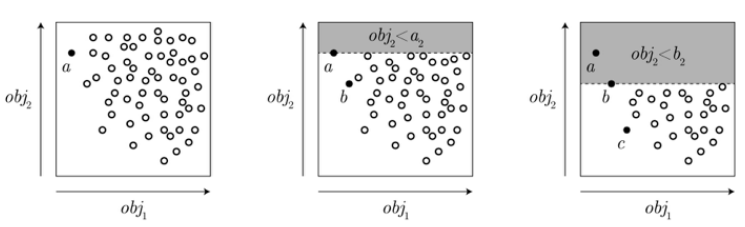
\includegraphics[width=10cm]{epsilon}
    \end{center}

    $\Rightarrow$ \begin{tabular}{l}
        Find the real pareto set\\
        Only for two objective\\
        $\epsilon$ should not be too small, but in practice it does not
        regenerate two times the same solution
    \end{tabular}

\end{itemize}

\subsubsection{Pareto set properties}
Sometimes it is too costly to compute the exact Pareto front. We
can use heuristic methods to approximate it (local search).

\begin{itemize}
    \item \textbf{Hyper-volume and diversified} 
        \begin{center}
            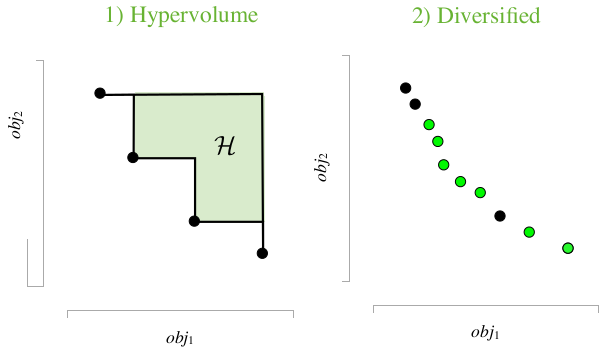
\includegraphics[width=8cm]{paretoProperties}
        \end{center}

    \item \textbf{Purity measure}
\end{itemize}


\subsection{Benchmarking optimization}

\begin{itemize}
    \item \textbf{Arithmetic mean of normalized results}: 
        \begin{enumerate}
            \item Assume that for each instance, we have
                measured the time required to reach optimality.
            \item Normalize them and check the result
                \begin{center}
                    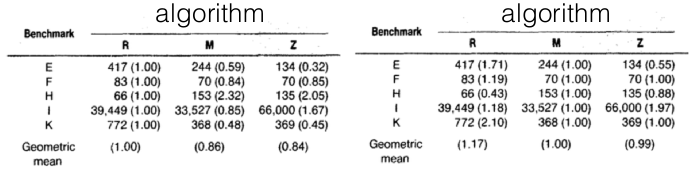
\includegraphics[width=11cm]{arithmetic}
                \end{center}

                Note, use \textbf{geometric mean} to have right 
                aggregate results (instead of average) : $\bigg(\prod_{n=1}^k
                x_n\bigg)^{\frac{1}{k}}$

        \end{enumerate}


    \item \textbf{Performance profiles}: $n_p$ instances for which we record various
        things for $n_s$ solvers. $t_{p,s}$ is th e time to solve $p$ by
        $s$.
        \begin{eqnarray*}
            \textrm{Performance ratio: } & \quad r_{p,s} &=
            \frac{t_{p,s}}{min\{t_{p,s}: s\in S\}}\\
            \textrm{Performance profile: } & \quad \rho_s(\tau)&=
    \frac{1}{n_p} \quad size \quad \{\quad p \in P: r_{p,s} < \tau\quad \}
    \end{eqnarray*}

    The performance profile is the probability for solver $s \in S$ to
    have a performance ratio within a factor $\tau$ of the best possible
    ratio. It's a cumulative distribution function of a performance
    metric.

    $\Rightarrow$ solvers with large probability $\rho_s(\tau)$ are to
    be preferred.
                \begin{center}
                    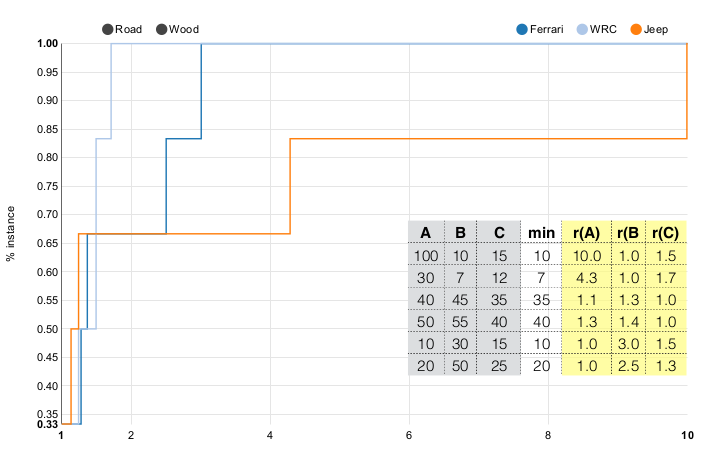
\includegraphics[width=11cm]{profiles}
                \end{center}



\end{itemize}


\subsection{Exam}
\begin{itemize}
    \item Multi-criteria optimization: Understand the three
        methods (lexicographic, weighted sum, Pareto-set).
    \item  Understand the dominance relations between
        solutions.
    \item  Be able to explain how to find a Pareto-set for a bi-
        objective problem.
    \item  Be able to explain why a weighted-sum method is not
        guaranteed to find the true Pareto-set.
    \item  Be able to build a performance profile and analyze it
\end{itemize}


\subsection{Discrete event simulation}
%TODO


